\chapter{Introduzione}

\section{Il Corso in Breve...}

\paragraph{Obiettivi:}

\begin{itemize}
\item Capire i concetti fondamentali del calcolo parallelo:
\begin{itemize}
  \item Sistemi paralleli. 
  \item Metriche, concetti, leggi fondamentali. 
  \item Approccio strutturato alla programmazione parallela. 
  \item Programmazione parallela di alto livello.
\end{itemize}
\item Scrivere codice parallelo efficiente su una macchina multicore (shared memory). 
\item Scrivere codice parallelo efficiente su un cluster di multicore (distributed memory). 
\item Scrivere codice parallelo efficiente su GPUs.
\end{itemize}

\paragraph{Percorso:}

\begin{itemize}
  \item Perché le performance sono importanti. 
  \item I princìpi della programmazione parallela.
  \item Approccio strutturato alla programmazione parallela. 
  \item Strumenti standard e di ricerca per la programmazione parallela. 
  \item Multicore e cluster.
\end{itemize}

\section{Il Parallel Computing}

\subsection{Perché si fa Parallel Computing?}

\qs{}{Che cos'è il Parallel Computing?}

\dfn{Parallel Computing}{
  Il \newfancyglitter{parallel computing} è la pratica di usare multipli processori per risolvere problemi più velocemente di quanto farebbe un singolo processore. Esso implica la capacità di: 
  \begin{itemize}
    \item Identificare ed esporre il parallelismo negli algoritmi e nei sistemi software. 
    \item Comprendere i costi, benefici e limiti di una determinata applicazione parallela. Alcuni codici potrebbero essere più efficienti con un'implementazione sequenziale.
  \end{itemize}
}

\paragraph{Esempi di macchine parallele:}

\begin{itemize}
  \item \fancyglitter{Cluster di Computer}: multipli computer indipendenti connessi con una o più reti ad alta velocità.
  \item \fancyglitter{SMP} (Symmetric Multi-Processor): multipli chip connessi a una gerarchia di shared memory.
  \item \fancyglitter{CMP} (Chip Multi-Processor, Multicore): multiple unità di computazione contenute su un singolo chip.
  \item \fancyglitter{GPUs} (acceleratori): come visto nel corso "Architetture degli Elaboratori II".
\end{itemize}

\paragraph{Le motivazioni del calcolo parallelo per \fancyglitter{aumentare le prestazioni}:}

\begin{itemize}
  \item Molto usate nella scienza e nelle simulazioni ingegneristiche. 
  \item Soprattutto per problemi troppo grandi per essere risolti su un singolo computer.
\end{itemize}

\nt{Per lungo tempo, il calcolo parallelo, è stato considerato una nicchia della computer science.}

\qs{}{Ma perché si vuole fare Parallel Computing oggi?}

\begin{itemize}
  \item Perché l'intera industria, attorno al 2004-2005, ha iniziato a spostarsi verso la computazione con multipli processori (multicore) in tutti i sistemi (laptops, desktops, workstations, servers, cellulari, dispositivi embedded). 
  \item Attualmente è una parte fondamentale del background di ogni computer scientist. 
  \item Lo spostamento verso i CMP ha certificato la fine della cosiddetta "\fancyglitter{Free Lunch Era}".
\end{itemize}

\subsection{Usi Recenti del Parallel Computing}

\begin{itemize}
  \item \fancyglitter{Big Data Analytics (BDA)}: 
    \begin{itemize}
      \item Dataset molto grandi (Terabyte, Petabyte, Exabyte). 
      \item Analisi in tempo reale.
    \end{itemize} 
  \item \fancyglitter{HPC and/for AI}:
    \begin{itemize}
      \item Utilizzo massivo di GPUs potenti. 
      \item HPC con framework ottimizzati per AI (TensorFlow, PyThorch,\dots).
    \end{itemize}
  \item Nel 1965, Gordon Moore (co-fondatore di Intel) predisse che la densità dei transistor sarebbe raddoppiata ogni 18 mesi (\fancyglitter{legge di Moore}). 
  \item Questo implica che sia possibile integrare sempre più transistor su un singolo chip. 
  \item Nel corso degli anni i chips dei microprocessori sono diventati sempre più piccoli, densi e potenti.
\end{itemize}

\paragraph{Implicazioni della legge di Moore:}

\begin{itemize}
  \item Il costo dei chips dei processori e delle memorie si è ridotto. 
  \item I processori sono diventati più veloci: 
    \begin{itemize}
      \item Transistor più piccoli e veloci. 
      \item Migliori microarchitetture, maggiori istruzioni per ciclo di clock. 
      \item Minori ritardi sulle porte logiche, più frequenza di clock. 
      \item Cache sempre più grandi per ridurre il collo di bottiglia di von Neumann. 
      \item Istruzioni SIMD.
    \end{itemize}
  \item Per cui, per molto tempo, si è pensato che la programmazione parallela fosse uno spreco in quanto sarebbe bastato aspettare un paio di anni.
\end{itemize}

\clm{}{}{
  Non conviene fare chip più grandi: 
  \begin{itemize}
    \item Aumenta il rischio che siano difettosi. 
    \item I segnali si trasferiscono troppo lentamente.
    \item Si ha troppo calore difficile da dissipare.
  \end{itemize}
}

\paragraph{Limiti del singolo chip:}

\begin{itemize}
  \item Il limite principale dell'aumento di prestazioni è dovuto a: 
    \begin{itemize}
      \item Velocità della luce (insormontabile). 
      \item Densità di potere (che aumenta ogni anno).
    \end{itemize}
  \item \fancyglitter{Legge scalare di Dennard}: nel 1974, Dennard osserca che l'aumento della densità di potere è costante con il fatto che i transistor diventano sempre più piccoli:
    \begin{itemize}
      \item Questo fu vero per quasi 30 anni. 
      \item Tra 2004-2005 si incontrò un muro all'aumento delle prestazioni.
    \end{itemize}
\end{itemize}

\paragraph{Muoversi verso i CMP per mantenere la densità di potere costante:}

$$\text{Power}_\text{dynamic} = \frac{1}{2}*C*V^2*F$$


$$\text{Perf} = \text{NCores}*F$$

\begin{itemize}
  \item V = voltaggio, C = capacitanza, F = frequenza di clock. 
  \item Ma V è circa F, quindi si può approssimare $\text{Power}_\text{dynamic} = C*F^3$.
  \item Se raddoppiamo il numero di core si raddoppia sia la potenza che  le performance.  
  \item Se raddoppiamo il numero di core e si dimezzano V e F si avrà la stessa performance, ma il potere si sarà ridotto di un fattore 4.
\end{itemize}

\nt{Nelle specifiche dei processori può venire indicata la frequenza di turbo, ossia la frequenza su un solo core in determinate condizioni di temperatura.}

\paragraph{Trend del CMP:}

\begin{itemize}
  \item I produttori di processori mettono multipli core su un solo chip. 
  \item La frequenza smette di crescere. 
  \item La legge di Moore è ancora valida, ma solo per quanto riguarda il numero dei cores. 
  \item Unità di cache sempre più grandi per il singolo chip. 
  \item La performance single-thread diventano sempre peggiori.
\end{itemize}

\begin{figure}[h]
  \centering
  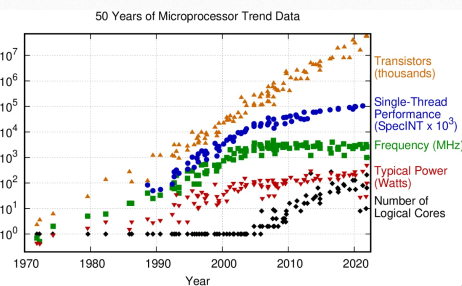
\includegraphics[scale=0.7]{01/trend.png}
  \caption{Trend dei microprocessori.}
\end{figure}

\paragraph{Multicore eterogenei:}

\begin{itemize}
  \item CMP integra diversi tipi di core su un singolo chip: CPU, GPU, DSP. 
  \item Power Efficiency: assegna differenti carichi di lavoro al tipo di core più appropriato per minimizzare lo spreco di energia. 
  \item Inoltre alcuni cores servono a massimizzare le prestazioni. 
\end{itemize}













